\section{Time Tracking}\label{sec:timetracking}
This section illustrates the teams time distribution for the project, as well as for each team member. We schedules a time difference between the two of us, as we had different curriculums this semester, with Jóhann able to spend more time than Hjalti on the project during the twelve week term. However during the three week term both team members were able to spend equal time on the project, as we had no other courses to divide our attention, which is why more time was spent on the project the last three weeks.

\subsection{Total time spent}
In figure \ref{fig:totaltime}, we can see a bar graph representing the time distribution over 17 weeks, where each bar represents a week, and it's height represents the amount of hours spent for each team member.

The reason for the decreased activity for two weeks is that the final exams were on during that period and the team needed a break from the project to study accordingly.

We scheduled 654 hours in total to devote to this project, and ended up spending in total 685 hours, due to increased work load and stress to get \emph{Project Discovery} ready for production. However, the team was happy with the hours spent and wished they could have done more.

\begin{figure}[H]
	\centering
	\graphicspath{ {./graphics/} }
    \centerline{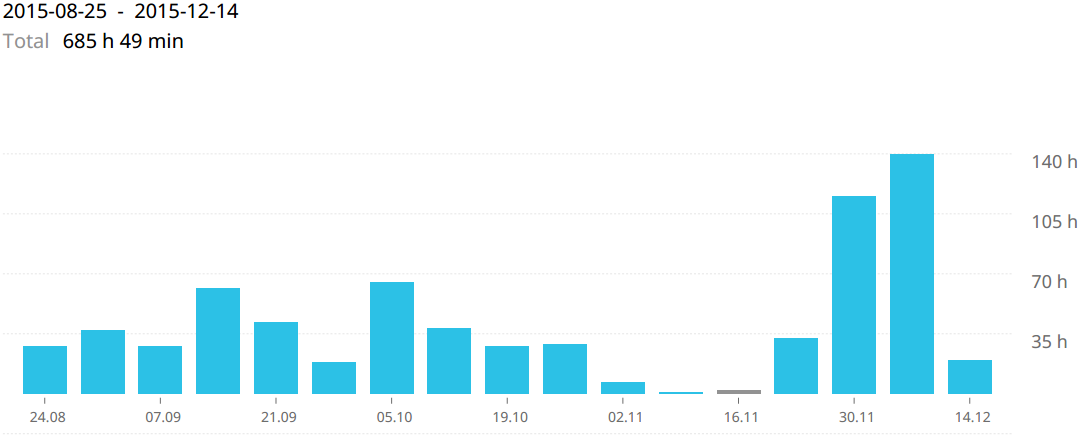
\includegraphics[scale=0.43]{total.PNG}}
    \caption{\label{fig:totaltime}Total time tracking breakdown.}
\end{figure}

\subsection{Time spent by Jóhann}
In figure \ref{fig:joitime}, we see a breakdown of the hours spent by Jóhann. He spent 347 hours, which slightly exceeded his original schedule of 342 hours.
\begin{figure}[H]
	\centering
	\graphicspath{ {./graphics/} }
    \centerline{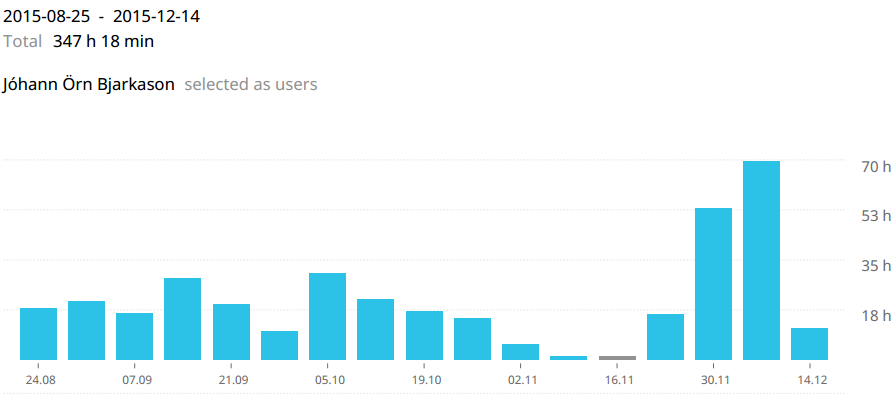
\includegraphics[scale=0.53]{joitime.PNG}}
    \caption{\label{fig:joitime}Time spent by Jóhann.}
\end{figure}

\subsection{Time spent by Hjalti}
In figure \ref{fig:hjaltitime}, we see a breakdown of the hours spent by Hjalti. He spent 338 hours, which exceeded his original schedule of 312 hours. 
\begin{figure}[H]
	\centering
	\graphicspath{ {./graphics/} }
    \centerline{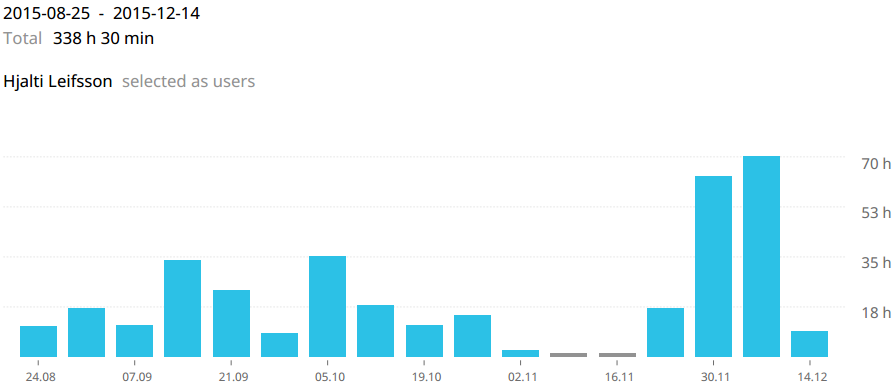
\includegraphics[scale=0.53]{hjaltitime.PNG}}
    \caption{\label{fig:hjaltitime}Time spent by Hjalti.}
\end{figure}